\section{Acceleration}
Rendering the triangle meshes quickly becomes a time intensive task, if the triangles forming the model are stored in a simple list. For example the scene shown in figure~\ref{fig:teapotWithAcc} consists of the Utah teapot standing on a plane, illuminated by a point light. Rendering it without an acceleration structure with enabled shadows takes approximately 1151 seconds or 19 minutes and 11 seconds. A first measure to improve matters is to surround the mesh with a box. Only if an incoming ray hits the box is it intersected with the triangles of the mesh. Using a bounding box reduces the rendering time to 613 seconds or about 10 min for scene~\ref{fig:teapotWithAcc}. To reduce computations required to render the scene further the number of intersection tests per pixel has to be reduced further. This can be done by subdividing the bounding box. Three different ways if subdivision will be considered. All of them start by finding the longest dimension of the box, but differ in the way this longest dimension is split.
\subsection{Middle-Split}
The first method splits the parent box into two children in the geometric middle of the longest axis. After the split the triangles are assigned to the
left or right subbox according to the position of their centroid. The two subboxes are then resized to ensure that no triangle vertices's lay outside the two boxes. After the resizing operation it is possible, that the two boxes overlap.   
\subsection{Split a sorted list}
The second method sorts the triangles contained in the box according to their centroid coordinate of the axis under consideration. The dimensions of the child boxes is then obtained by splitting the sorted list in the middle and assigning each child half of the triangles. The new boxes are then resized such that they contain all of their triangles entirely.
\subsection{Surface area heuristic}
Finally the surface area heuristic is considered, which splits along several points and chooses from a set of available options by evaluating the cost function:
\begin{equation}
\text{cost} = N_{\text{left}} \cdot \frac{S_{left}}{S_{total}} +
              N_{\text{right}} \cdot \frac{S_{right}}{S_{right}}
\end{equation}
Where $N$ denotes the number of primitives in a given box and $S$ its surface along the dimension under consideration. Before the cost function can be evaluated the parent box is split along its longest edge $c_{SAH}$ times, and $c_{SAH} + 1$ child boxes are created. The child boxes of each side of the cut are then combined and resized and the cost function is evaluated for each combination. Finally the combination with the lowest cost is chosen. 

\subsection{Intersection testing}
In order to avoid unnecessary computation work it is important to avoid intersecting boxes, where a visible hit cannot be found. To do this a ray is always intersected with the box having the centroid closer to the camera. The second box is only considered if an intersection found in the first box lies in a space where both boxes overlap. 

\subsection{Results}
Table~\ref{tab:teapodTiming} shows the timing results of the three implemented splitting methods. Considering the decrease from the initial 10 minutes the reduction of rendering time is impressive for each method. The surface area heuristic is the best choice here as its tree is the most efficient and the additional time needed to construct it does not make a difference in this example. Table~\ref{tab:DragonTiming} shows the situation for the dragon scene. Here the surface Area heuristic is still the most efficient in terms of rendering time, but it looses during the tree generation phase. This would certainly change if the implementation of the SAH tree generation function would be optimized further.  

\begin{table}
\centering
\begin{tabular}{|c|c|c|c|c|} \hline
				& read[s] & split[s] & render[s] & total[s] \\ \hline
Middle-Split    & 0.16 & 0.95  & 23.61  & 24.72	\\
Sort-Split      & 0.17 & 0.06  & 30.47  & 30.7	\\
SAH             & 0.16 & 0.18  & 17.27  & 17.61	\\ \hline
\end{tabular}
\caption{Time measurments taken using various splitting methods when rendering the teapot scene.}
\label{tab:teapodTiming}
\end{table}

\begin{figure}
\centering
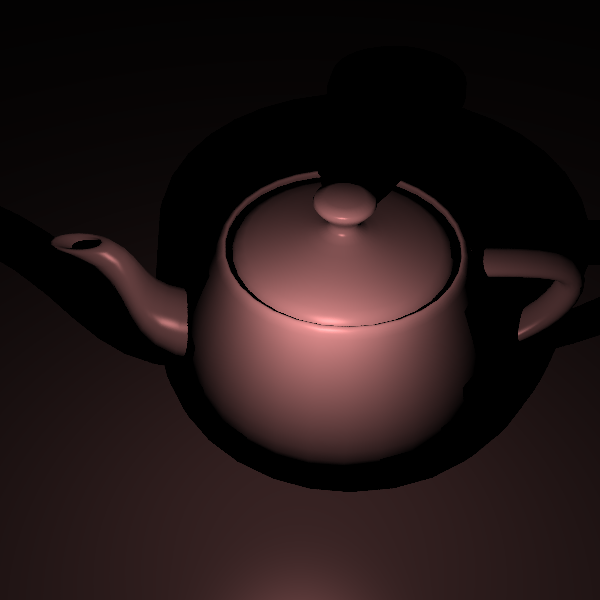
\includegraphics[width=0.45\linewidth]{./img/teapot}
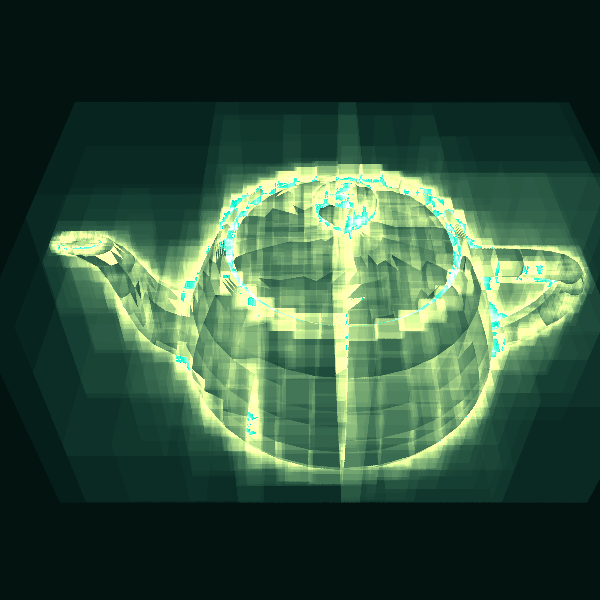
\includegraphics[width=0.45\linewidth]{./img/teaFCGreen10}
\caption{Utah-Teapot rendered image and false color visualizations of the intersections with a color map maximum at 180 intersections, with 10 SAH cuts per split.}
\label{fig:teapotWithAcc}
\end{figure}

\begin{table}
\centering
\begin{tabular}{|c|c|c|c|c|} \hline
				& read[s] & split[s] & render[s] & total[s] \\ \hline
Middle-Split    & 11.4 & 3.7   &  10.53  & 25.63 \\
Sort-Split      & 10.6 & 4.6   &  20.5  & 35.7	 \\
SAH             & 11.0 & 14.3  &  6.71  & 32.01	 \\ \hline
\end{tabular}
\caption{Time measurments taken using various splitting methods when rendering the stanford dragon scene.}
\label{tab:DragonTiming}
\end{table}


\begin{figure}
\centering
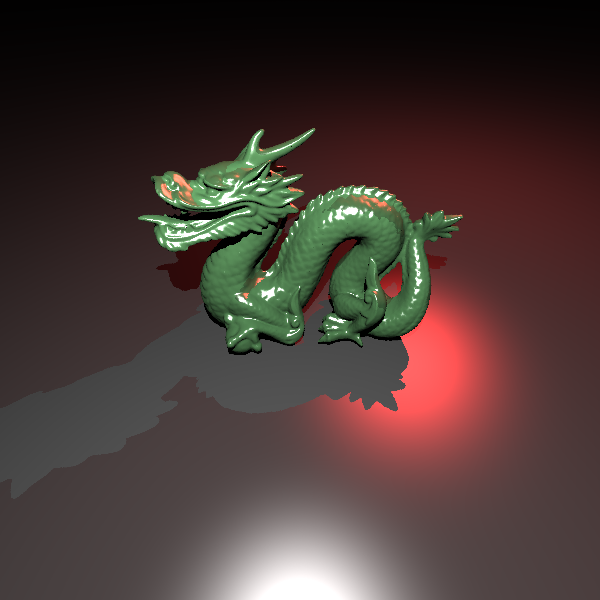
\includegraphics[width=0.45\linewidth]{./img/dragon}
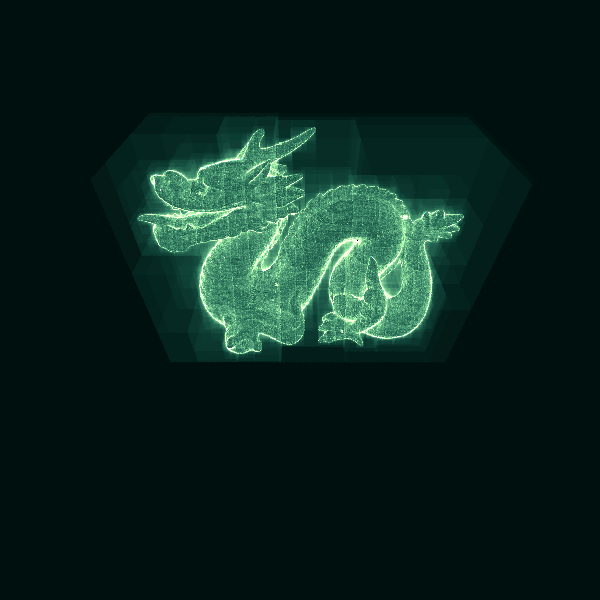
\includegraphics[width=0.45\linewidth]{./img/dragonFC4}
\caption{High resolution Standford-Dragon rendered image and false color visualizations of the intersections with a color map maximum at 180 intersections and 4 SAH cuts per split }
\label{fig:dragon}
\end{figure}


\section{Textures}
In order to use textures each object hit point has the be associated with coordinates in the $u,v$ texture space. For wavefront (\texttt{.obj}) these coordinates come from a data file along with the triangle-mesh data. It is important to note that the coordinate system for wavefront objects is located at the top left of the image file. With that in mind textures, which sometimes come shipped along with \texttt{.obj}-files can be used. An apple texture is shown in figure~\ref{fig:apple}. In the same image a procedural texture is used for the plane. 
\begin{figure}
\centering
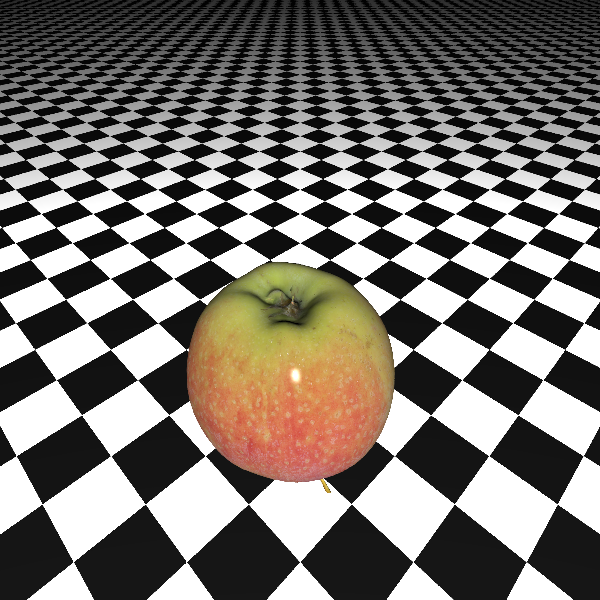
\includegraphics[width=0.45\linewidth]{./img/apple}
\caption{Apple on chessboard}
\label{fig:apple}
\end{figure}
\subsection{Procedural texturess}
The chess-board like pattern is generated by dividing the $u$ and $v$ coordinate by the desired size of the rectangles. If the rounded results of the division are added and the modulo with two is computed every point can be associated with one or zero. Which serves as the criterion to choose the texture color. 
\subsubsection{Julia-set textures}
More interesting patterns can be computed by using fractals. Often used examples are Julia fractals found from functions of the form:
\begin{equation}
f(z) = z^2 + c \;\;\; z \in \mathbb{C}
\end{equation}
Where $c$ is considered the seed. Changing $c$ changes the appearance of the fractal drastically. Julia sets are generated by applying the function $f(z)$ to itself repeatedly, compute $f(z),f(f(z)),f(f(f(z))),\dots$. This process is repeated until the iteration exceeds a predefined limit value $\|z_n|\ > k$, or a maximum number of iterations is reached. Each point is then colored according to how many iterations $n$ it took to reach the limit $k$. The logarithm of the iterations counter is hashed linearly from 0 to the largest occurring value to colors. Plots with $c = -0.07,0.652, c = -0.02,0.652, c= -0.02,0.8$ with the initial $z_{\text{init}} \in [-1,1]$ and $k = 1$ are given in figure~\ref{fig:julia4}.
\begin{figure}
\centering
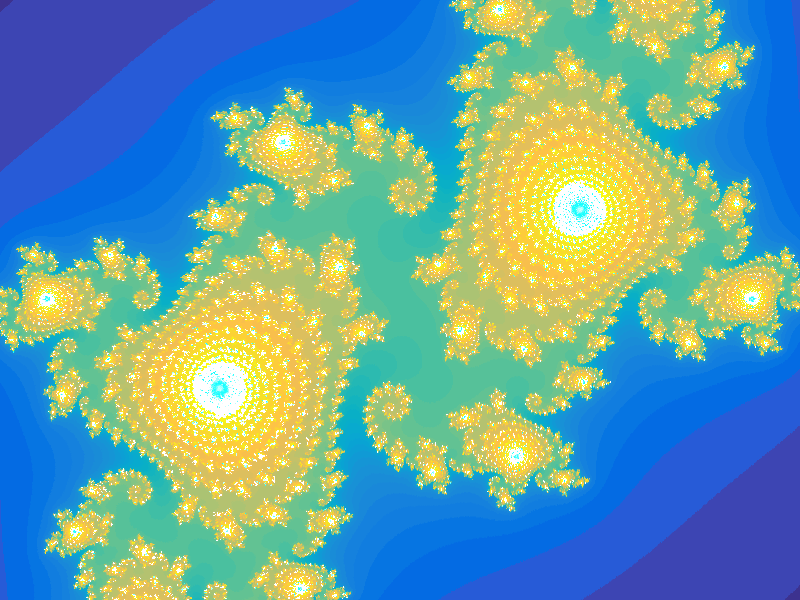
\includegraphics[width=0.25\linewidth]{./img/julia1New}
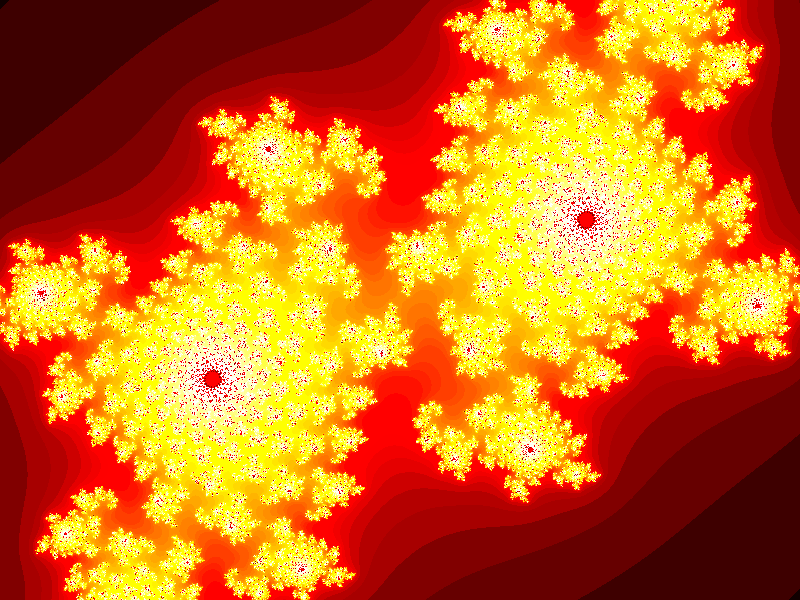
\includegraphics[width=0.25\linewidth]{./img/julia2}
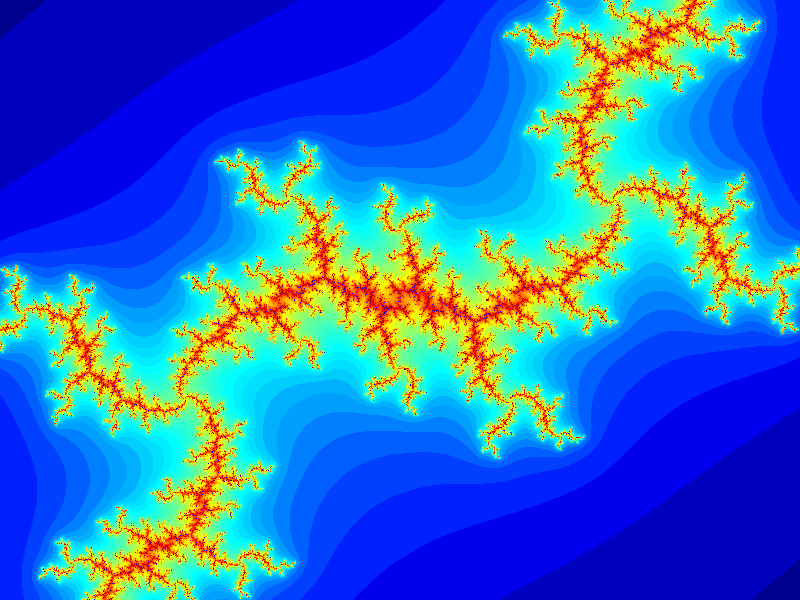
\includegraphics[width=0.25\linewidth]{./img/julia4}
\caption{Julia fractals using different seeds and colormaps.}
\label{fig:julia4}
\end{figure}

\subsubsection{Function meshes}
To obtain a 3d visualization of a function, a triangle mesh can be computed from grid data. The mesh can be set up by assembling triangles following the rule:
\begin{align}
p_1 &= \{x[i],y[j],f_n(x[i]\cdot y[j]\}			\\
p_2 &= \{x[i+1],y[j],f_n(x[i+1] + i\cdot y[j])\}		\\
p_3 &= \{x[i],y(j+1),f_n(x[i]+i\cdot y[j+1])\}		\\
p_4 &= \{x[i+1],y(j+1),f_n(x[i+1]+i\cdot y[j+1]\}	\\
\text{tri}_1 &= \{p_1,p_2,p_4\} \\
\text{tri}_2 &= \{p_1,p_4,p_3\} \\
\end{align}
Which is assuming that the $x$ and $y$ values are stored in vectors and that $f_n$ has been stored in a two dimensional matrix-array. Then the meshes' triangles
can be constructed by looping over the expressions outlined above. The triangle vertices are stored in a counterclockwise order. Thus the normals follow from equation~\ref{eq:triNormal}. The result of setting up such a mesh consisting of $(2*(N-1))^2$ with $N = 800$ triangles using the inverse value of the logarithmic iteration counter as z-coordinate is shown in figure~\ref{fig:fractalValleyMap}. A top down view is shown on the left and a 3d perspective view computed from intersecting the mesh on the right.

\begin{figure}
\centering
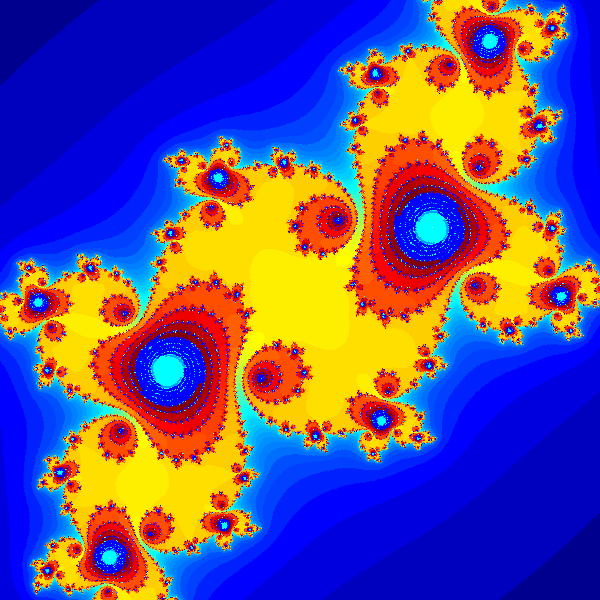
\includegraphics[width=0.45\linewidth]{./img/fractalValleyMap}
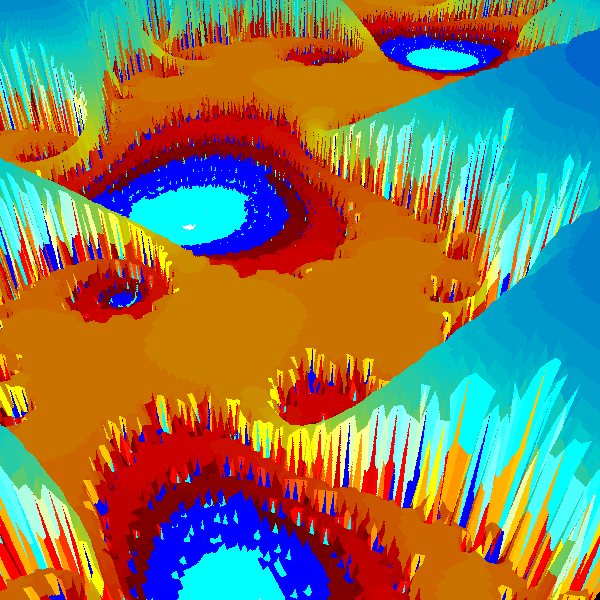
\includegraphics[width=0.45\linewidth]{./img/fractalValley}
\caption{Top and 3d view of the Julia fractal computed from $f(z) = z^2 + c$ with $c = -0.1,0.651$.}
\label{fig:fractalValleyMap}
\end{figure}


